%TODO: make all more concise, bullet points

\begin{frame}
	\frametitle{Project Background}
	Nuclear fusion -- the energy of the future!
    \vspace{10pt}
	\begin{itemize}
	    \item Must produce and contain an extremely hot and dense plasma
	    \begin{itemize}
		    \item Magnetic Confinement Fusion (MCF): toroidal circulation
		    \item Inertial Confinement Fusion (ICF): spherical compression
		\end{itemize}
		\vspace{10pt}
		\item Modern designs require enriched Hydrogen fuel of two varieties:
	    \begin{itemize}
		    \item Deuterium ($^2$H) -- abundant in naturally-sourced water.
		    \item Tritium ($^3$H) -- extremely rare, but can be produced \textit{in-reactor}.
		\end{itemize}
	\end{itemize}
	\vspace{10pt}
	\centering{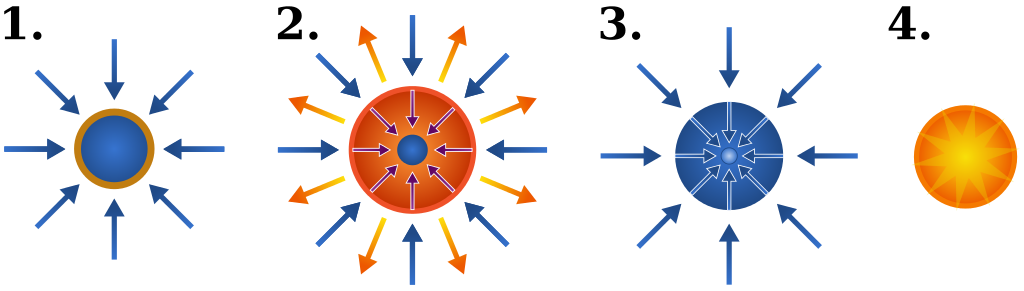
\includegraphics[height=3cm]{icf_diagram}}
\end{frame}

\begin{frame}
	\frametitle{Problem Description}
	Tritium breeding blankets convert neutron radiation to tritium fuel:
	\begin{align*}
		\isotope[1][0]{n} + \isotope[6][3]{Li} \rightarrow \isotope[3][1]{H} +
		\isotope[4][2]{He}
		\qquad\qquad
		\isotope[1][0]{n} + \isotope[7][3]{Li} \rightarrow \isotope[3][1]{H} +
		\isotope[4][2]{He} + \isotope[1][0]{n}
	\end{align*}
	Tritium breeding ratio (TBR) = fuel bred / fuel consumed
	
	\begin{itemize}
	    \item Depends on numerous geometric and material parameters.
	    \item Evaluated precisely by OpenMC neutronics simulation \textit{Paramak}, but is computationally expensive. 
	\end{itemize}
	
	\vspace{15pt}
	
	\begin{block}{Our Challenge:}
		\begin{center}
			Produce a fast TBR function that strongly approximates Paramak, making use of the latest in surrogate modelling techniques.
		\end{center}
	\end{block}
\end{frame}

\begin{frame}
	\frametitle{Data Generation}
	We produced training and test datasets by uniform random sampling over the 7 discrete and 11 continuous parameters of Paramak.\newline
	 \begin{columns}[onlytextwidth,T]
      \column{\dimexpr\linewidth-7cm-5mm}
        
        Paramak was deployed on UCL's Hypatia cluster:
        \begin{itemize}
            \item Generated 1M samples.
            \item 27 days of runtime.
        \end{itemize}
        
        	\vspace{10pt}
        
        Two classes of runs:
        \begin{itemize}
            \item All parameters free.
            \item Discrete fixed, continuous free.
        \end{itemize}
        
      \column{7cm}
      \vspace{-0.5cm}
      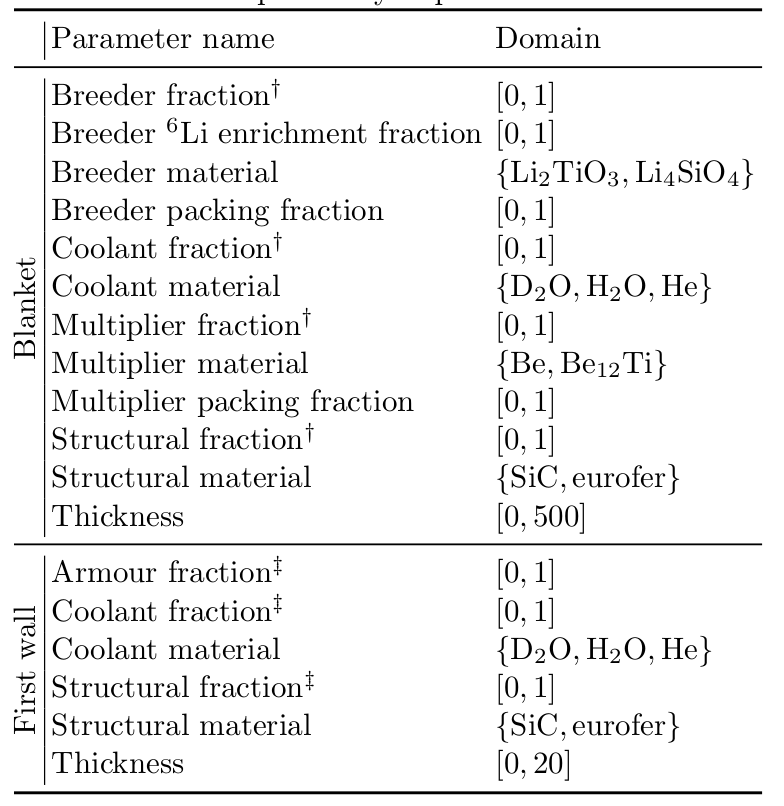
\includegraphics[trim={0 0 0 2mm},clip,width=7cm]{params}

    \end{columns}
\end{frame}

%\begin{frame}
%	\frametitle{Dimensionality Reduction}
%	\begin{itemize}
%		\item % TODO
%	\end{itemize}
%\end{frame}

\begin{frame}
	\frametitle{Methodology}
		Conventional regression task -- search for a cheap surrogate $\hat{f}(x)$ that
		minimizes dissimilarity with an expensive function $f(x)$:

		\begin{itemize}
			\item
				Regression performance: mean absolute error, $\sigma$ of
				error, $R^2$, $R^2_\text{adj.}$
			\item
				Computational complexity:
				training \& prediction time / sample
		\end{itemize}

		\vspace{2em}

		2 approaches for surrogate training:
		\begin{enumerate}
			\item
				Decoupled -- trains models from previously sampled
				datapoints.
			\item
				Adaptive -- repeats sampling \& model training, increases
				sampling density in low-performance regions.
		\end{enumerate}
\end{frame}

